%! Author = domore
%! Date = 8/11/21

% Preamble
\documentclass[11pt]{article}

% Packages
\usepackage{amsmath}
\usepackage{graphicx}
\usepackage{hyperref}
\hypersetup{
    colorlinks=true,
    linkcolor=blue,
    filecolor=magenta,
    urlcolor=cyan,
    citecolor=blue
}
\usepackage{cleveref}
\usepackage[margin=1.1in]{geometry}
\usepackage{python}
\usepackage{pythontex}
\usepackage{pdfpages}
% Documentation
% https://raw.githubusercontent.com/gpoore/pythontex/master/pythontex/pythontex.pdf
% tricks
% https://raw.githubusercontent.com/gpoore/pythontex/master/pythontex_gallery/pythontex_gallery.tex
% compilation
%pdflatex -aux-directory=/home/domore/PycharmProjects/ds_project-1/document_files/aux -output-directory=/home/domore/PycharmProjects/ds_project-1 main_document.tex
%python document_files/pythontex/pythontex3.py document_files/main_document.tex
%pdflatex -aux-directory=/home/domore/PycharmProjects/ds_project-1/document_files/aux -output-directory=/home/domore/PycharmProjects/ds_project-1 main_document.tex
\usepackage[framemethod=TikZ]{mdframed}
\usepackage{booktabs}
%\usepackage{multirow}
\usepackage{rotating}

% for future projects
% \usepackage[usefamily=juliacon]{pythontex}

% Document
\begin{document}


\includepdf[pages={2}]{src/titlepage.pdf}

\tableofcontents\newpage

\part{Learning phase} \label{part:learning}

\section{Introduction}\label{sec:introduction}
In the paragraphs to come we will discuss different approaches and models to be used in the dataset used in~\cite{wine}.

The following dataset consist of different a sample of wines with different characteristics and their relevant
quality.
The box below has an overview description of the dataset we will analyse.
A further description of each variable can be found in \Cref{tab:description_wine}.

% these lines will not be presented in the pdf
% pyconcode only excecutes (does not show code)
%! suppress = EscapeUnderscore
%! suppress = EscapeHashOutsideCommand
\begin{pyconcode}
import pandas as pd
import os
import numpy as np

# Referencing folders and data names
path = os.getcwd()
# We have to re-structure the path since we are in LaTeX
path = os.path.abspath(os.path.join(path, os.pardir))
file_name = 'winequality-red.csv'
path_file = f'{path}/code_python/project1_wine/data/{file_name}'
# We load the data and present an overview
wine_data = pd.read_csv(path_file)
\end{pyconcode}

%! suppress = EscapeUnderscore
%\begin{pyconsole}[][frame=single]
\begin{pyconsole}[][]
wine_data.info()
wine_data.describe().round(decimals=2).transpose()
\end{pyconsole}

\section{Exploratory analysis}\label{sec:exploratory-analysis}

To avoid unnecessary analysis, first we will perform a few checks to get a deeper understanding of the
data we are using.
To that end, we first check that the correlation structure amongst the variables (see \cref{fig:wine_heatmap}),
including the quality of the wine.
This should give us a general idea of how and if the variables are related to one another.


\begin{figure}[h!]
    \centering
    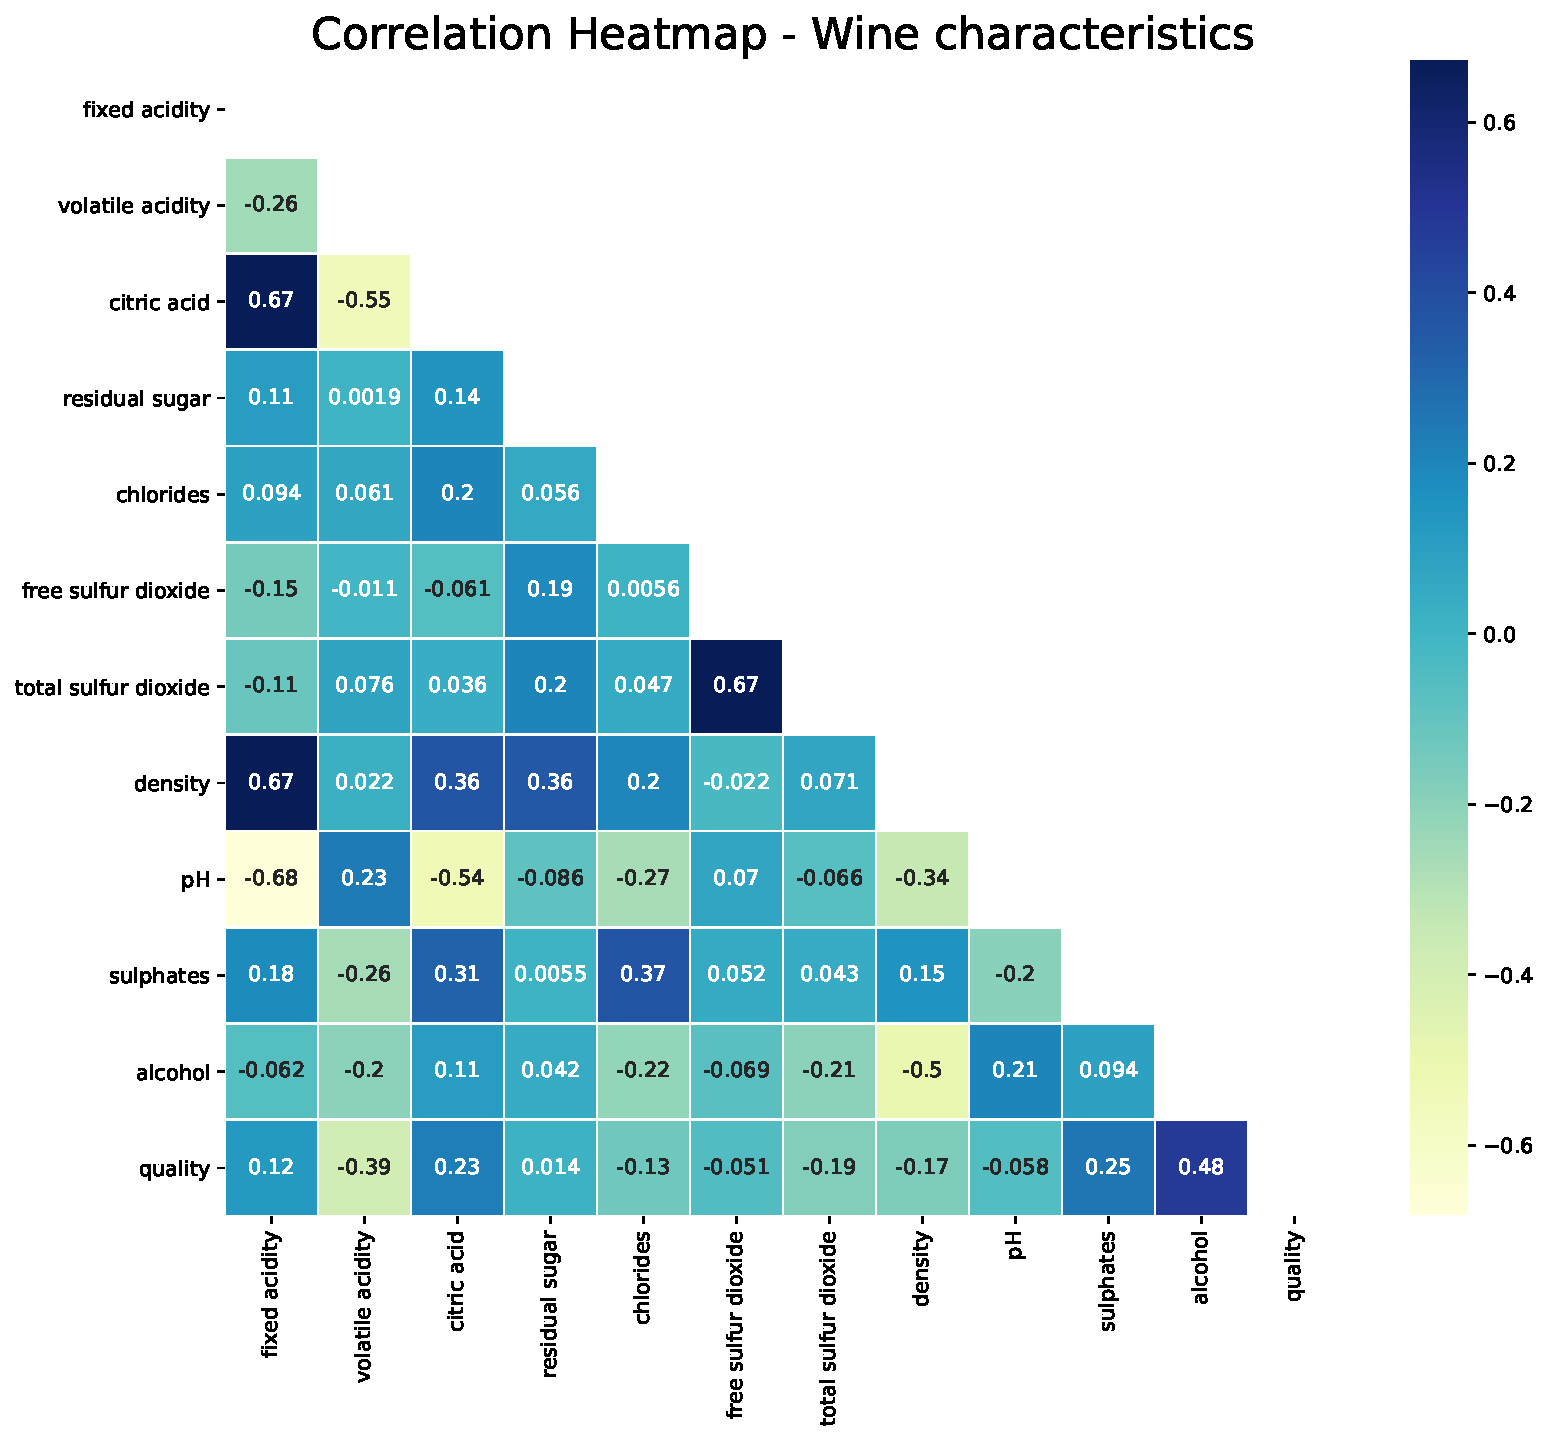
\includegraphics[width=0.9\textwidth]{figs/wine_heatmap}
    \caption{Correlation structure of wine characteristics.}
    \label{fig:wine_heatmap}
\end{figure}


There are a few things we could check in the data to assess whether what we are looking relates somehow
to our prior knowledge about the topic.
This prior knowledge might help us identify certain links, that might not be obvious if the data were not labelled.

At first glance, one can note that \emph{fixed acidity} and \emph{citric acidity} are strongly correlated (negatively) to the \emph{pH},
although their correlation is not \emph{-1}.
This should relate to our prior knowledge, given that \emph{pH} is directly related to the acidity of a
solution.
Additionally, we can see that \emph{alcohol} correlates negatively with the \emph{density} of the wine.
This makes sense, given that the wine is a solution of different solutes, those in all likelihood are ``heavier''
than the alcohol solute, as well as the water solvent which is definitely ``heavier'' than alcohol.
Hence, the more the alcohol content increases in the wine, the less dense it becomes.
Another interesting characteristic of the wine that is highly correlated to its quality is the
alcohol content.

\vspace{2pt}
Another visual analysis we could perform are KDEs (Kernel Density Estimates).
These, we could imagine as a cross-sectional cut in a bi-variate probability distribution.
\Cref{fig:wine_kdes} shows us that even though the wines in the sample range from quality 3 to 8
(see histogram subplot in row 3, column 4), it would seem that there are mostly 4 important groups.
The earlier stated fact, ad priori, provide us with a key insight we should have in mind when trying
to fit any kind of model.
I.e., the tails of the quality (grades 3 and 8) will be underrepresented, then most models we could think
of fitting will have trouble predicting a grade close to 3 and 8 and beyond (to each direction).

\begin{figure}[h!]
    \centering
    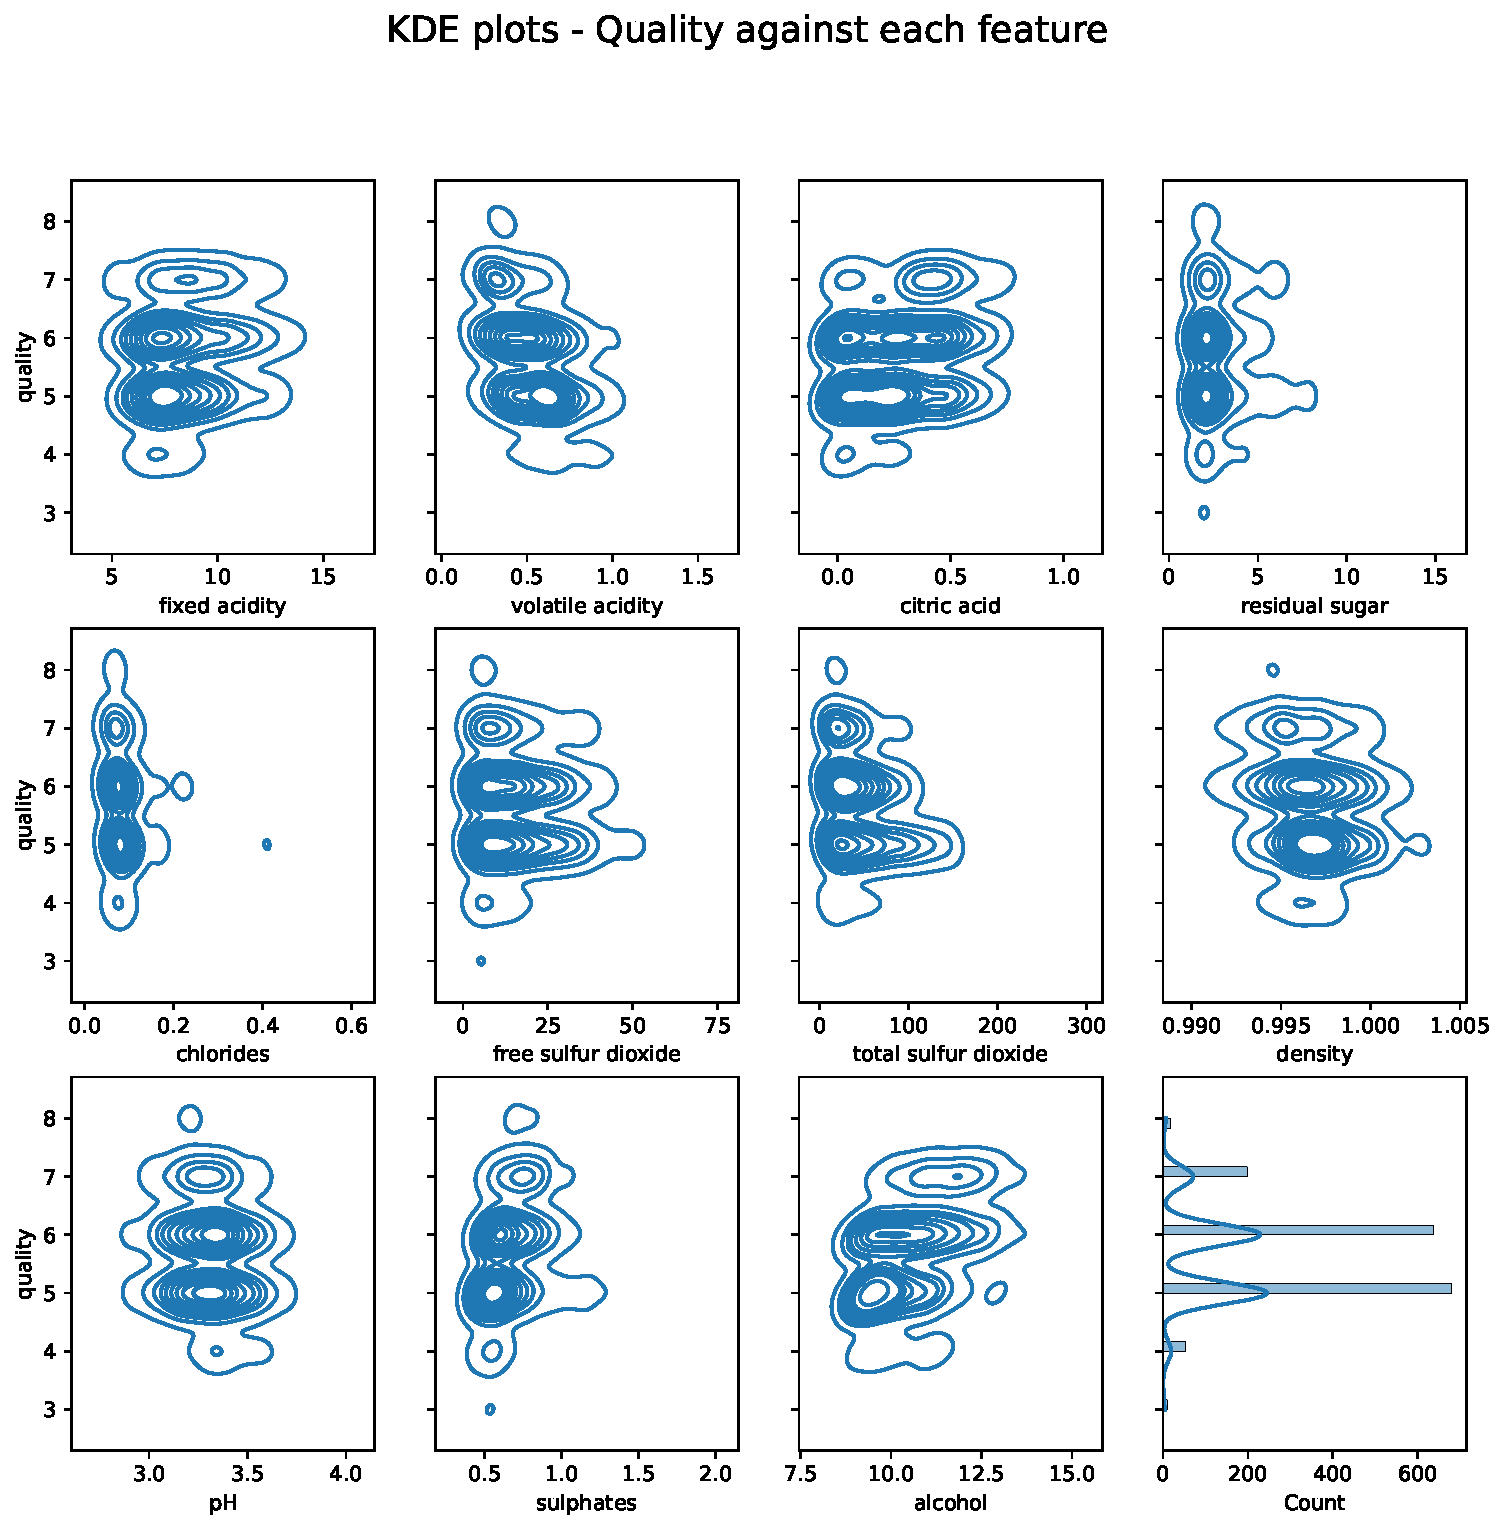
\includegraphics[width=0.9\textwidth]{figs/wine_kde}
    \caption{KDEs for wine features.}
    \label{fig:wine_kdes}
\end{figure}


\section{Analyses}\label{sec:analyses}

Among the many features that we could analyse in these data\footnote{Some other analyses, like clustering the wine sample do
carry the same importance. I.e., we could try clustering the wine sample, to find that certain
wines belong or were produced by the same vineyard due to the similarities in the grapes which
will most likely relate to their characteristics when turned into wine.
Even though this might be interesting, it is not as useful to a researcher/data scientist trying to add value
to the winemaking processes.}, we will stick to predicting the quality
of a wine given its characteristics.

To predict the quality of the wines, we will use all possible available features\footnote{Could be that using all
features decreases the predictive power of certain models. But these we could only find out through thorough investigation
which is out of the scope in this project.} and split our database: 80\% of the data will be used for training and
the remaining 20\% will be used for testing and computing assessment metrics.
To achieve this, we will mostly use \emph{sci-kit learn} library and sub-libraries.

%! suppress = EscapeUnderscore
%! suppress = EscapeHashOutsideCommand
\begin{pyconsole}[][]
# Pre-processing
# Shaping data
X = wine_data.drop('quality', axis=1)
y = wine_data['quality']
# Defining a seed for shuffling the data
seed = 123
# Splitting data into train/test.
from sklearn.model_selection import train_test_split
X_train, X_test, Y_train, y_test = train_test_split(X, y, test_size=0.20,
                                                    random_state=seed)
\end{pyconsole}

After splitting our initial sample into train and test, we proceed to standardize it.
Although this is not absolutely necessary, there are some models we will use in the following that
have better performance and provide better estimates\footnote{Less prone to be biased.}.
Then, some models will use the standardized data, and some others (like in \emph{tree regression})
will not.

%! suppress = EscapeUnderscore
%! suppress = EscapeHashOutsideCommand
\begin{pyconsole}[][]
# Converting 1D arrays to dataframe
y_train = pd.DataFrame(Y_train, columns=['quality'])
# Scaling training samples
from sklearn.preprocessing import StandardScaler
train_X_scaler = StandardScaler()
train_Y_scaler = StandardScaler()
# we first fit the training data to different scaling objects
# to keep track of them
train_X_scaler.fit(X_train)
train_Y_scaler.fit(y_train)
x_train = train_X_scaler.transform(X_train)
y_train = train_Y_scaler.transform(y_train)
\end{pyconsole}

It is important to note that the scaling (standardization) is only performed in the \textbf{training sample}.
Then, when we have our predictions from the models in the \emph{scaled space}, we will revert them back
to the \emph{observation space} using the inverse scaling we determined on the train sample.
This is of high importance when trying to build a predictive model.
If we used the scaling from the test sample, we would be \emph{snooping into the data}, which would probably
increase the models' accuracy (artificially), but with the power of \emph{hindsight}.

In the following snippets, code of the fitting will be provided.
After all models are presented, the results will be shown, and some discussion stemming from them will be
held.

\subsection{Linear Regression}\label{subsec:linear-regression}

%! suppress = EscapeUnderscore
%! suppress = EscapeHashOutsideCommand
\begin{pyconsole}[][]
# Linear Regression
# Normal Linear Regression (L2 Norm)
from sklearn.linear_model import LinearRegression as lr

# We first initialise the model and then fit with the training obs.
normal_lr = lr(fit_intercept=True, normalize=False)
normal_lr.fit(X=x_train, y=y_train)
# Predicting values, we first need to transform the X_test matrix
# using our earlier defined scale
nlr_y = normal_lr.predict(train_X_scaler.transform(X_test))
# Reverting our predicted values to their level using the scale determined
# from the training sample
nlr_y = train_Y_scaler.inverse_transform(nlr_y)
\end{pyconsole}

\subsection{Lasso Regression}\label{subsec:lasso-regression}
%! suppress = EscapeUnderscore
%! suppress = EscapeHashOutsideCommand
\begin{pyconsole}[][]
# Lasso Linear Regression (L1 Norm)
# we do not standardize here otherwise the lasso regression might turn
# all coefficients to 0 only to use the intercept.
from sklearn.linear_model import Lasso as lasso

# We first initialise the model and then fit with the training observations
# also do not use intercept, if the intercept is allowed, again makes
# most of the coefficients to be 0.
lasso_lr = lasso(fit_intercept=False, normalize=False)
lasso_lr.fit(X=X_train, y=Y_train)
lassolr_y = lasso_lr.predict(X_test)
\end{pyconsole}
\newpage
\subsection{Neural Networks}\label{subsec:neural-networks}

%! suppress = EscapeUnderscore
%! suppress = EscapeHashOutsideCommand
\begin{pyverbatim}[][]
# Neural Network - using sklearn
from sklearn.neural_network import MLPRegressor

NN_scikit = MLPRegressor(random_state=seed,
                         max_iter=500,
                         hidden_layer_sizes=(22,),
                         activation='logistic').fit(x_train,
                                                    np.ravel(y_train))
NN_scikit.out_activation_ = 'identity'
# we use (22,) in the hidden layers to try to capture the features and
# their interactions, we will do it because it is too little data.
# Using more neurons or hidden layers in this case might induce
# over-fitting, given the small sample size.
nn_scikit_y = NN_scikit.predict(train_X_scaler.transform(X_test))
# Reverting our predicted values to their level using the scale determined
# from the training sample.
nn_scikit_y = train_Y_scaler.inverse_transform(nn_scikit_y)
\end{pyverbatim}

%! suppress = EscapeUnderscore
%! suppress = EscapeHashOutsideCommand
\begin{pyverbatim}[][]
# NN With Keras
from keras.models import Sequential
from keras.layers import Dense
import tensorflow as tf
tf.random.set_seed(seed)


def squared_loss(y_true, y_pred):
    squared_difference = tf.square(y_true - y_pred)
    return tf.reduce_sum(squared_difference, axis=-1)  # Note the `axis=-1`


nn_keras_tf = Sequential()
nn_keras_tf.add(Dense(22,
                      input_dim=11,  # expects 11 inputs
                      activation='sigmoid'))
nn_keras_tf.add(Dense(1, activation='linear'))  # output layer
# since we are using keras to call TF we need to compile the model we
# designed in keras for it to be into the TF framework.
# print(dir(tf.keras.optimizers))
# print(dir(tf.keras.losses))
# print(dir(tf.keras.metrics))
nn_keras_tf.compile(loss=squared_loss, optimizer='adam')
nn_keras_tf.fit(x_train, y_train, epochs=500)
nn_keras_tf_y = train_Y_scaler.inverse_transform(
                nn_keras_tf.predict(train_X_scaler.transform(X_test)))
\end{pyverbatim}

\subsection{Regression Tree}\label{subsec:regression-tree}

%! suppress = EscapeUnderscore
%! suppress = EscapeHashOutsideCommand
\begin{pyverbatim}[][]
# Regression Tree
from sklearn.tree import DecisionTreeRegressor

tree_model = DecisionTreeRegressor(max_depth=4)
# Data without scaling.
tree_model.fit(X_train, Y_train)
tree_y = tree_model.predict(X_test)
\end{pyverbatim}

\subsection{Support Vector Regression (SVR)}\label{subsec:support-vector-regression-(svr)}

%! suppress = EscapeUnderscore
%! suppress = EscapeHashOutsideCommand
\begin{pyverbatim}[][]
# SVM (Regression)
from sklearn.svm import SVR

svr = SVR()
svr.fit(x_train, np.ravel(y_train))
svr_y = train_Y_scaler.inverse_transform(svr.predict(
                                        train_X_scaler.transform(X_test)))
\end{pyverbatim}


\section{Results}\label{sec:results}

Most of the models used in \Cref{sec:analyses} were fitted using \emph{sk-learn} libraries.
This was done just for ease of quick prototyping and implementation, but for production models, probably
other libraries would be preferred, if not outright developing some of them from scratch.
One model, one neural network, was additionally fitted with the \emph{keras} library to emphasize that the results
should be quite similar, however not identical\footnote{There are several reasons why almost two identically defined
models can have different outputs, in particular when it comes to neural networks. Some of these factors are the
solvers used, the number of epochs, learning rate and steps, tolerances and staring points.}.

%\caption{Description of wine characteristics.}
\begin{table}[h!]
\centering
\caption{Metric comparison different competing models.}
\label{tab:model_results}
\begin{tabular}{lrrr}
\toprule
{} &  RMSE &  MAPE &  Score \\
\midrule
linear regression       &  0.66 &  0.10 &   0.34 \\
lasso linear regression &  0.73 &  0.10 &   0.20 \\
NN Scikit               &  0.65 &  0.10 &   0.36 \\
NN Keras TF             &  0.64 &  0.09 &   0.38 \\
Regression Tree         &  0.69 &  0.10 &   0.28 \\
SVR                     &  0.61 &  0.08 &   0.44 \\
\bottomrule
\end{tabular}
\end{table}


%\label{tab:model_results}

\Cref{tab:model_results} shows the results of different loss functions and score for the different competing models.
Let us quickly define each of the metrics.

\begin{equation}
  \mathrm{RMSE} = \sum_{i=1}^{d}
  \left(\frac{y_{i}-\hat{y}_{i}}{y_{i}}
  \right)^2.
\label{eq:rmse}
\end{equation}

\begin{equation}
  \mathrm{MAPE} = \sum_{i=1}^{d}
  \left|\frac{y_{i}-\hat{y}_{i}}{y_{i}}
  \right| \cdot 100\%.
\label{eq:mape}
\end{equation}

\begin{equation}
  \mathrm{Score} = 1 - \frac{\sum_{i=1}^{d}(y_{i}-\hat{y}_{i})^2}{\sum_{i=1}^{d}(y_{i}-\bar{y})^2}.
\label{eq:score}
\end{equation}

Where $y_{i}$ is the true $i^{\text{th}}$ observation in the test sample, $\hat{y}_{i}$ is the forecasted
$i^{\text{th}}$ observation and $\bar{y}$ denotes the average value of the test sample.

After observing the values in \cref{tab:model_results}, one can see a clear winner in terms of the loss
metrics, i.e.\ the SVR model which has the lowest RMSE and MAPE out of the competing models as well as
the largest Score out of the models in scope.

Another fact we can observe is that the MAPE is $0.1$ for most of the models, although this is just due the
rounding of results to 2 decimal places.

Also, if we compared the two more classic regressions: Linear regression, and the \emph{lasso} regression,
we find that it would seem the latter to be of inferior performance than the former.
This was to be expected, given that the \emph{lasso} regression penalises the amount of regressors when
more systematic error could still be extracted by using more regressors.\ By the same token, the \emph{lasso}
regression looks to find a sparser model, which is useful when one tries to make sense of a model with fewer
variables, and hence easier to control for and to explain.

When comparing the neural network models, we can observe that both models perform quite similarly.
They do not output exactly the same results even when trying to match their parametrisation and hyper-parameters,
as one can observe in \cref{subsec:neural-networks}.
This is also to be expected from models like neural networks, since they are initialised (pseudo)randomly, hence
the (stochastic) gradient descent algorithm can output widely different results with the same inputs, just by
factors like starting points (in particular when the starting points are \emph{close} in \emph{input space} to a
local minimum) and initial shuffling of the sub-samples to initialise the algorithm.




\section{Discussion}\label{sec:discussion}

So far, we have covered quantitatively the results in terms of the loss metrics.
If we had stopped here, then we should have concluded that the SVR model was superior to the rest of the models,
and therefore we should use this model in the future.

However, as it was hinted in \cref{sec:exploratory-analysis}, it would be probably wise to investigate the distribution
of the predictions.
This should give us a better picture of the \emph{output space} the models are able to map/span.
Let us have a look at the distribution of the predictions of each model and compare them to the
distributions. \Cref{fig:prediction_hists} shows the different histograms with the relative frequency of the
predictions (the relative frequency histograms for the train/test sample are in read for easier identification).

\begin{figure}[h!]
    \centering
    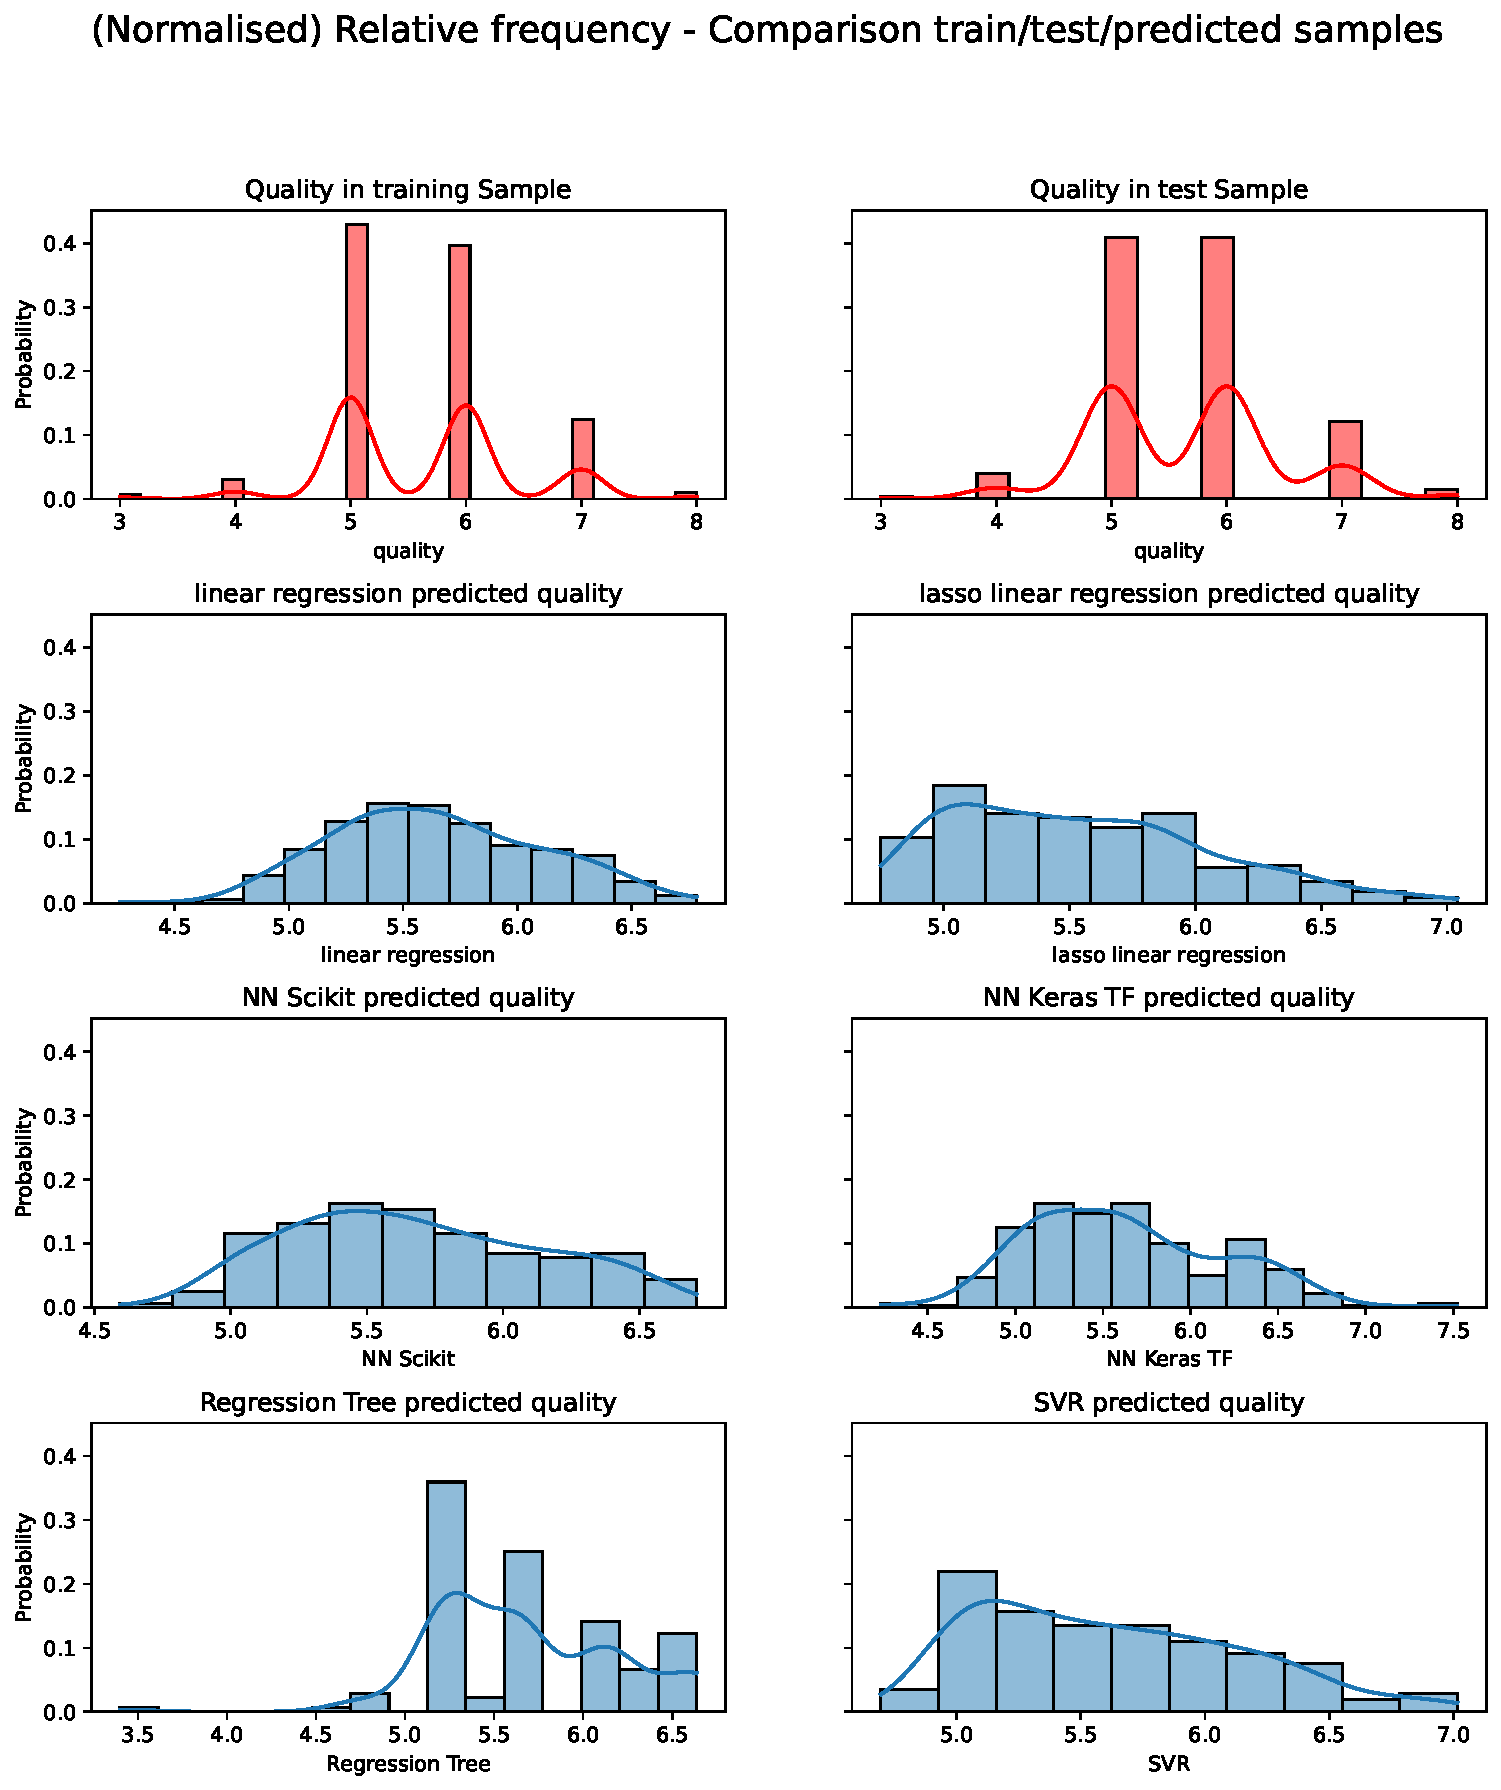
\includegraphics[width=0.9\textwidth]{figs/prediction_histograms}
    \caption{Relative frequency histograms for train/test and predicted samples.}
    \label{fig:prediction_hists}
\end{figure}

As we can observe in \cref{fig:prediction_hists}, both train and test sample seem to be quite similar in terms
of distribution, meaning the distribution of the train sample represents well (in relative terms) the test one.
This means that a model that is fitted with the train data should be able to output more or less similarly values
in the same distribution.

From the distribution of the train and test sample one can clearly observe a bimodal pattern with a slight
biased towards the higher quality grades.
When it comes to the models' predictions we see some major differences in the outline (density) shape.
Most models have a single mode, except for the predictions obtained with the regression tree, where it somewhat
unclear given the clusters.
The fact of that most distributions are unimodal is understandable.
Given that both modes in the original samples are in the consecutive grades (in an ordinal classification scale), and
that the models output continuum values.
This can be observed in most models having their mode at about the value $5.5$.

If we go back to the initial winner model (SVR), we can see that the outline does not represent well the test sample
distribution, it does however pick even the slight bias towards lower grades of the training sample.
In fact, the distribution of the predictions coming from the SVR model has a bias towards lower grades, in particular
the grade 5, which tells that the model fitted quite well the distribution of the training sample and new data even
with high grades is not able to offset this initial fit.

Nevertheless, we see that most, if not all the models' predictions seem to be around the values $5-6$.
So let us explore what happens in the \emph{tail} grades (either very low or very high grades).

\subsection{Explanability} \label{subsec:explanability}

Let us analyse the SHAP (Shapley Additive Explanations) waterfall fo(r a few of the \emph{tail} predictions of two
different models: normal linear regression (see \cref{subsec:linear-regression}, \cref{fig:shap_nlr}) and SVR
(see \cref{subsec:support-vector-regression-(svr)}, \cref{fig:shap_svr}).

The following graphical analyses show the additive contribution of the features in a model to each prediction, starting
from a base prediction (\emph{average}) to the particular prediction.

\subsubsection{Linear regression}\label{subsubsec:linear-regression}
\begin{figure}[h!]
    \centering
    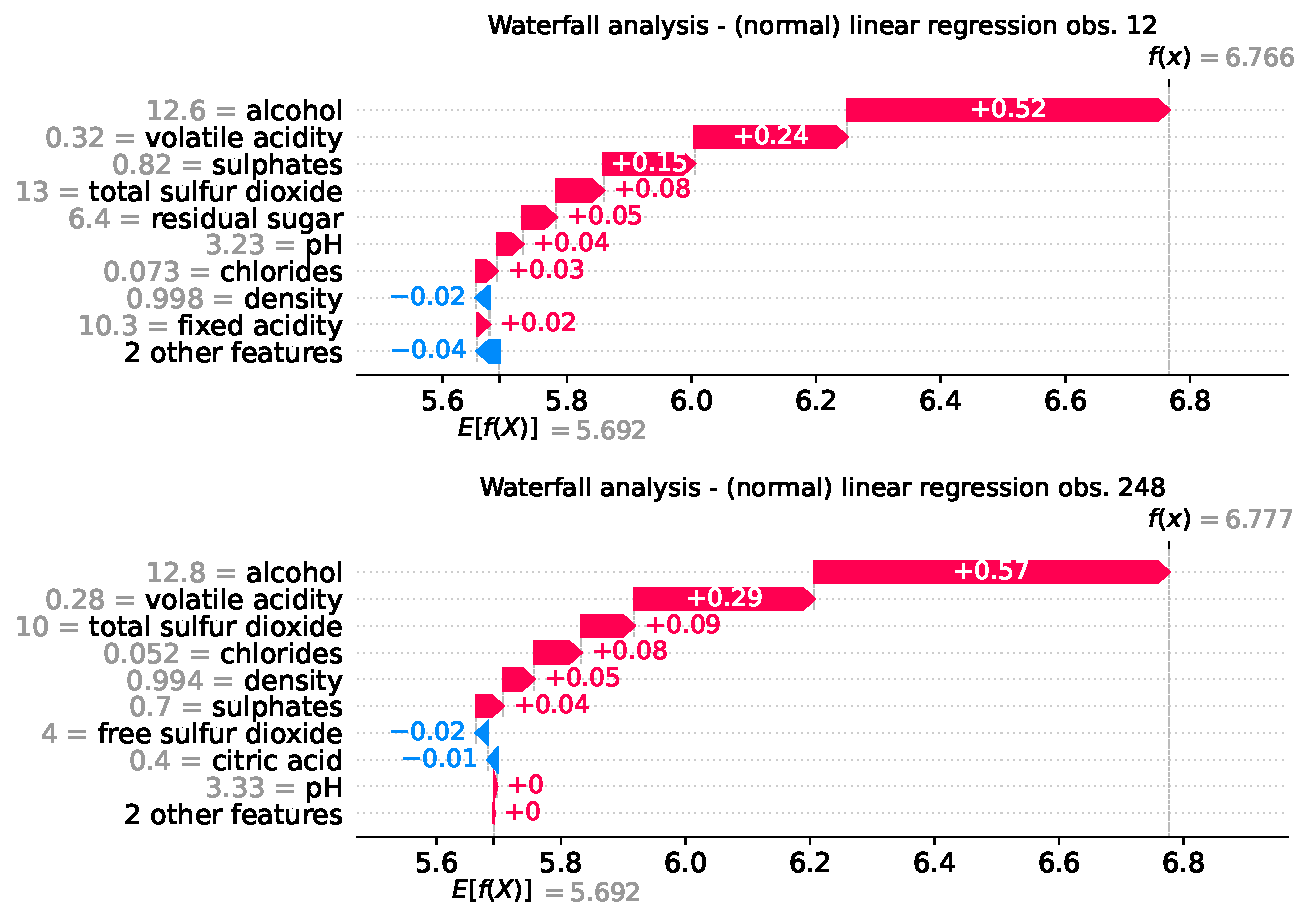
\includegraphics[width=0.9\textwidth]{figs/shape_nlr}
    \caption{(SHAP) Waterfall analysis of predictions - Normal linear regression (two similar predictions).}
    \label{fig:shap_nlr}
\end{figure}

If we analysed \cref{fig:shap_nlr}, we can see the both observations (predictions) 12 and 248 using the normal
linear model output a very similar value: $6.766$ and $6.777$, respectively.
If we looked in more detail we see that for similar values of several variables (alcohol, volatile acidity,
total sulfur dioxide, sulphates and chlorides) their contributions stay consistent.
This more or less tells the reader that two similar observations (wine features) would produce a similar
prediction, which is good if we are trying to build a robust model.

If for example, we pay close attention to the density of the wine we can see that for these two predictions, even having
similar density values, their contribution to the grade (quality) changes in sign, which suggests us that given our model
a value in between $0.998$ and $0.994$ is the threshold for a zero contribution to a better/lower grade (meaning that
a density value below this threshold would increase the quality of the wine, the inverse being also true), all else being
equal (\emph{ceteris paribus}).

\subsubsection{SVR}

If we observe now the winning model (see \cref{fig:shap_svr}), we can say similar things as we said for the linear model in
\cref{subsubsec:linear-regression} in terms of the consistency of the individual contributions.
Although, for this model, we can note one large difference that does not occur for the linear model, i.e., that
the pH being the same for both observations provides a different contribution towards the particular prediction.
This shows us that the SVR model picks more subtleties in the underlying data and not just linear terms.

The latter fact has certain pros and cons.
For example, picking up relationships that are not just linear might uncover certain links amongst the features,
providing a better view on possible positive or negative synergies in the underlying characteristics of the wine.
As a con, the researcher could not know \emph{ad priori} whether similar characteristics would output similar grades.
\begin{figure}[h!]
    \centering
    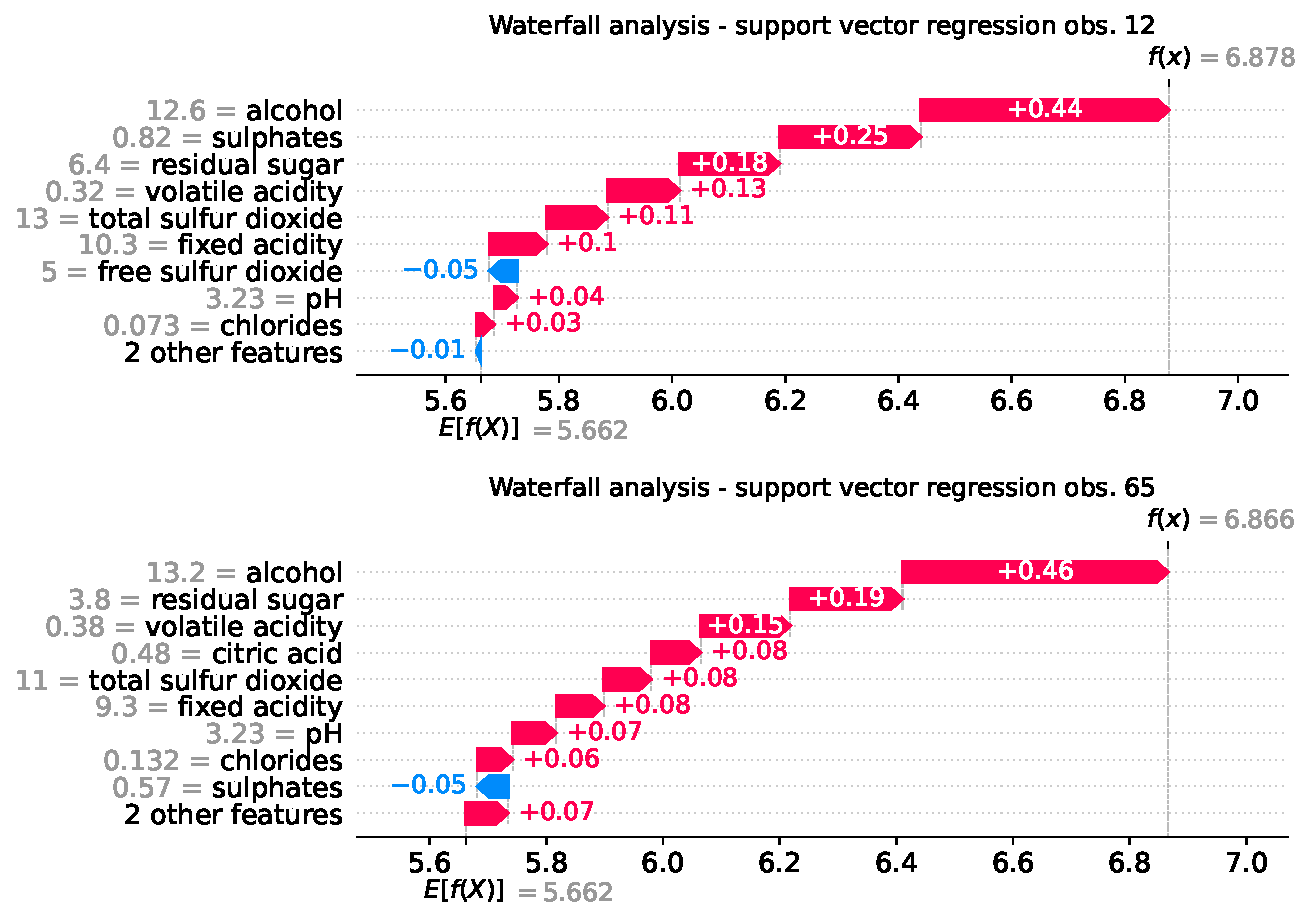
\includegraphics[width=0.9\textwidth]{figs/shape_svr}
    \caption{(SHAP) Waterfall analysis of predictions - Support vector regression (two similar predictions).}
    \label{fig:shap_svr}
\end{figure}


\subsection{Retro-feedback}\label{subsec:retro-feedback}

So far we have looked at different models and tried to analyse which model performs better than the others.
We defined that if we were using only the loss metrics as the indicator for better performance, then the SVR model
would be a clear winner.

However, after checking the prediction distributions in \cref{fig:prediction_hists}, we became uncertain on whether a
model like SVR or linear regression could provide us with a reliable mechanism to predict quality grades that are on the
tail of initial quality distribution in the training sample.
Moreover, the waterfall analysis displayed in \cref{fig:shap_svr}, showed us that the pH feature contributed in different
magnitude for the same pH value.

\vspace{1pt}

What we have encountered thus far are the typical problems a researcher/data scientist has when trying to develop models
for predicting pretty much anything.

\subsection{Decision}\label{subsec:decision}

For what is next, we will only continue the analysis and predictions of the two models: (normal) linear regression
(linear regression from now on), and the SVR model.

Even though we could continue with the other 4 models, we will focus only on the two mentioned models for the sake of
simplicity.
In particular given that the SVR model was the winner by loss metrics and because the ease of interpretation of the
linear model.



\part{Calibrating phase} \label{part:calibrating}

\section{Outlines}\label{sec:outlines}

% todo pre-processing by clustering, then fit models based on cluster to get more granularity of less frequent grades

\section{Clustering}\label{sec:clustering}

\subsection{Checking clusters}\label{subsec:checking-clusters}

\subsection{Calibrating models}\label{subsec:calibrating-models}


\part{Experimental phase} \label{part:experimenting}

\section{Simulation study}\label{sec:simulation-study}

% todo explain how to bypass the issue of the distribution tails when forecasting on new data either ensamble models or local approximations.

% todo implement a solution for this issue, first clustering observation features, then fitting multiple models depending on which clusters provide a better fit.

% todo how to add value -> add noise in many directions to obsevations caring not to overstep boundaries for certain variables like pH and make a consensus with the models
% to see whether it is possible to find some 'key' characteristics that make a good wine.

\part{Wrapping up, conclusions} \label{part:conclusions}


%{\color{red}\textbf{[1]}}
All these characteristics are important in a wine.
We used all these statistical models to try to understand to which degree they are important
to determine a wine`s quality.
These analyses might be really important for a winemaker to know.
Given that by affecting the inherent characteristics of the wine will most likely have an
impact on the quality of that wine.





\begin{thebibliography}{1}
\bibitem{wine} P. Cortez, A. Cerdeira, F. Almeida, T. Matos and J. Reis. {\em Modeling wine preferences by data mining from physicochemical properties.
In Decision Support Systems, Elsevier, 47(4):547-553},  2009.
\end{thebibliography}


\clearpage
\begin{sidewaystable}
    \centering
    \caption{Description of wine characteristics.}
    \resizebox{\columnwidth}{!}{
    \begin{tabular}{ll}
\toprule
      Characteristic &                                                                                                                                                                                      Description \\
\midrule
       fixed acidity &                                                                                                                most acids involved with wine or fixed or nonvolatile (do not evaporate readily). \\
    volatile acidity &                                                                                         the amount of acetic acid in wine, which at too high of levels can lead to an unpleasant, vinegar taste. \\
      citric acidity &                                                                                                                  found in small quantities, citric acid can add "freshness" and flavor to wines. \\
      residual sugar &                     the amount of sugar remaining after fermentation stops, it`s rare to find wines with less than 1 gram/liter and wines with greater than 45 grams/liter are considered sweet. \\
           chlorides &                                                                                                                                                                  the amount of salt in the wine. \\
 free sulfur dioxide &                                the free form of SO2 exists in equilibrium between molecular SO2 (as a dissolved gas) and bi-sulfate ion; it prevents microbial growth and the oxidation of wine. \\
total sulfur dioxide & amount of free and bound forms of S02; in low concentrations, SO2 is mostly undetectable in wine, but at free SO2 concentrations over 50 ppm, SO2 becomes evident in the nose and taste of wine. \\
             density &                                                                                               the density of water is close to that of water depending on the percent alcohol and sugar content. \\
                  pH &                                                          describes how acidic or basic a wine is on a scale from 0 (very acidic) to 14 (very basic); most wines are between 3-4 on the pH scale. \\
           sulphates &                                                                         a wine additive which can contribute to sulfur dioxide gas (S02) levels, which acts as an antimicrobial and antioxidant. \\
             alcohol &                                                                                                                                                         the percent alcohol content of the wine. \\
             quality &                                                                                                                                 output variable (based on sensory data, score between 0 and 10). \\
\bottomrule
\end{tabular}


    }
    \label{tab:description_wine}
\end{sidewaystable}





\end{document}